\documentclass[aspectratio=169]{beamer}

\usepackage{ccicons}
\usepackage{fontspec}
\usepackage{import}
\usepackage{listings}
\usepackage{tikz}

\subimport{../}{colors.tex}

\usetikzlibrary{
  arrows,
  arrows.meta,
  automata,
  backgrounds,
  calc,
  chains,
  decorations.pathreplacing,
  fit,
  matrix,
  overlay-beamer-styles,
  positioning,
  shapes,
  tikzmark,
}
\usetikzmarklibrary{listings}

\hypersetup{
  colorlinks=true,
  urlcolor=uclablue,
}

\setbeamercolor{frametitle}{fg=primarycolor}
\setbeamercolor{structure}{fg=primarycolor}
\setbeamercolor{enumerate item}{fg=black}
\setbeamercolor{itemize item}{fg=black}
\setbeamercolor{itemize subitem}{fg=black}

\setbeamersize{text margin left=26.6mm}
\addtolength{\headsep}{2mm}

\setbeamertemplate{navigation symbols}{}
\setbeamertemplate{headline}{}
\setbeamertemplate{footline}{}
\setbeamertemplate{itemize item}{\color{black}}
\setbeamertemplate{itemize items}[circle]

\setbeamertemplate{footline}{
  \begin{tikzpicture}[remember picture,
                      overlay,
                      shift={(current page.south west)}]
    \node [black!50, inner sep=2mm, anchor=south east]
          at (current page.south east) {\footnotesize \insertframenumber};
  \end{tikzpicture}
}

\setsansfont{Overpass}[Scale=MatchLowercase]
\setmonofont{Overpass Mono}[Scale=MatchLowercase]

\makeatletter
\newcommand\version[1]{\renewcommand\@version{#1}}
\newcommand\@version{}
\def\insertversion{\@version}

\newcommand\lecturenumber[1]{\renewcommand\@lecturenumber{#1}}
\newcommand\@lecturenumber{}
\def\insertlecturenumber{\@lecturenumber}
\makeatother

\setbeamertemplate{title page}
{
  \begin{tikzpicture}[remember picture,
                      overlay,
                      shift={(current page.south west)},
                      background rectangle/.style={fill=uclablue},
                      show background rectangle]
    \node [anchor=west, align=left, inner sep=0, text=white]
          (lecturenumber) at (\paperwidth / 6, \paperheight * 3 / 4)
          {\Large Lecture \insertlecturenumber};
    \node [inner sep=0, align=left, text=white, node distance=0,
           above left=of lecturenumber, anchor=south west, yshift=2mm]
          {\Large CS 111: Operating System Principles};
    \node (title) [inner sep=0, anchor=west, align=right, text=white]
          at (\paperwidth / 6, \paperheight / 2)
          {{\bfseries \Huge \inserttitle{}}};
    \node [inner sep=0, align=right, text=white, node distance=0,
           below right=of title, anchor=north east, yshift=-1mm]
          {{\footnotesize \ttfamily \insertversion}};
    \node [inner sep=0, text=white, align=left, anchor=west]
          (author) at (\paperwidth / 6, \paperheight / 4)
          {\insertauthor};
    \node [text=white, inner sep=0, align=left, node distance=0,
           below left=of author, anchor=north west, yshift=-2mm]
          {\insertdate};
    \node [align=right, anchor=south east, inner sep=2mm, text=white]
          (license) at (\paperwidth, 0)
          {\footnotesize This  work is licensed under a
           \href{http://creativecommons.org/licenses/by-sa/4.0/}
                {\color{uclagold} Creative Commons Attribution-ShareAlike 4.0
                 International License}};
    \node [text=white, inner sep=0, align=right, node distance=0,
           above right=of license, anchor=south east, xshift=-2mm]
          {\Large \ccbysa};
  \end{tikzpicture}
}

\tikzset{
  >=Straight Barb[],
  shorten >=1pt,
  initial text=,
}

\lstset{
  basicstyle=\footnotesize\ttfamily,
}


\lecturenumber{14}
\title{Disks}
\version{3.0.0}
\author{Jon Eyolfson}
\date{November 16, 2021}

\begin{document}
  \begin{frame}[plain, noframenumbering]
    \titlepage
  \end{frame}

  \begin{frame}{The Structure of a Hard Disk Drive (aka HDD)}
    \begin{center}
        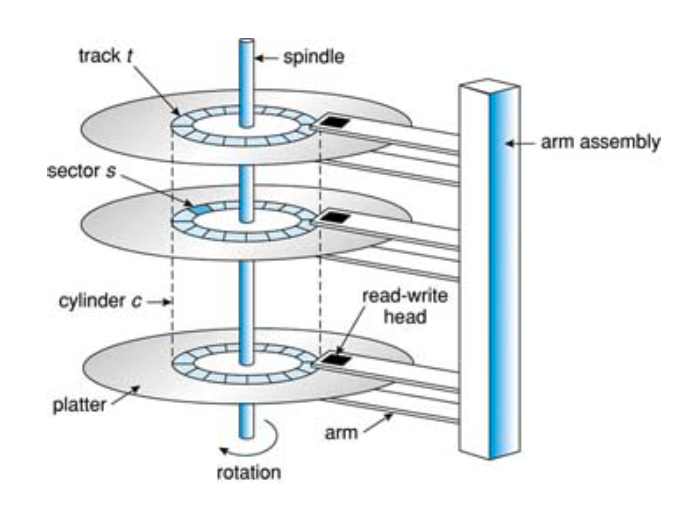
\includegraphics[height=0.8\textheight]{hdd1.png}
    \end{center}
  \end{frame}

  \begin{frame}{Access Speed Depends on Locality}

    Sectors on same track can be read continuously

    \vspace{2em}

    Switching tracks needs repositioning of the arm

    \hspace{2em} Repositioning the arm is expensive)
  \end{frame}

  \begin{frame}{You Physically Address a HDD Using Cylinder-Head-Sector (CHS)}

    Data has the following Coordinates (multi-dimensional polar coodinates):

    \begin{itemize}
      \item Platter: which revolving platter (addressed as head) [z Axis]
      \item Track: which track lane on platter (historically cylinder) [$||r||$]
      \item Sector: which sector on track [$\Theta$]
    \end{itemize}

    \vspace{2em}

    The historical CHS has an approximate 8 GB limit of addressable space

    \hspace{2em} (512 bytes/sector)×(63 sectors/track)×(255 heads (tracks/cylinder))

    \hspace{2em} ×(1024 cylinders)

    \vspace{2em}

    LBA (Logical Block Addressing) uses one number to address

    any block and is not limited to 8~GB
  \end{frame}

  \begin{frame}{Shingled Magnet Recording (SMR)}

    The write head only writes in the center of a track, and has unused padding

    \vspace{2em}

    You can't write to this padding without destroying neighboring tracks

    \vspace{2em}

    SMR however, allows you to write over the padding, if you do it sequentially

    \vspace{2em}

    Drive performance may suffer, but it's easier to increase capacity 

    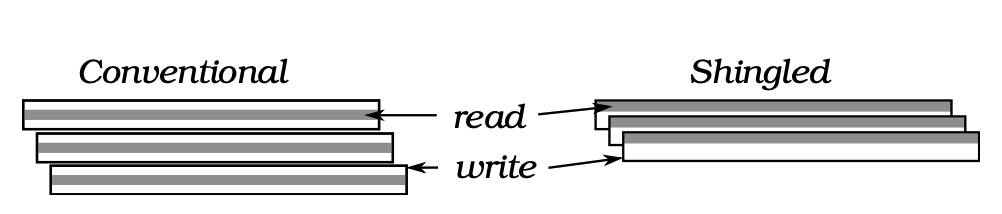
\includegraphics[height=20mm]{hdd2.png}
  \end{frame}

  \begin{frame}{HDDs Have Latencies Dependent on the Distance Travelled}

    Rotational delay: physically rotate the disk to get to the correct sector

    \hspace{2em} Typically 4-8 ms (average delay is half of a full rotation)

    \vspace{2em}

    Seek time: moving the disk arm to get to the correct track

    \hspace{2em} Typically 0.5-2 ms

    \vspace{2em}

    Transfer time: how long it takes to read bytes from the disk

    \hspace{2em} Typically the maximum transfer speed is 125 MB/s
  \end{frame}

  \begin{frame}{Calculating Transfer Rate}

    The total time, $\mathsf{T}$, is equal to

    \hspace{2em} rotational delay + seek time + transfer time

    \vspace{2em}

    The transfer rate, $\mathsf{R}$, is equal to

    \hspace{2em} Size of the transfer / $\mathsf{T}$

    \vspace{2em}

    What is the transfer rate of

    \hspace{2em} Large sequential accesses?

    \hspace{2em} Small random accesses?
  \end{frame}

  \begin{frame}{We Should Use HDDs Sequentially Whenever Possible}
    \begin{tabular}{lll}
                       & HDD 1     & HDD 2      \\
      Rotational speed & 7,200 RPM & 15,000 RPM \\
      Rotational latency (ms) & 4.2 & 2.0 \\
      Average seek (ms) & 9 & 4 \\
      Max transfer & 105 MB/s & 125 MB/s \\
      Platters & 4 & 4 \\
      Interface & SATA & SCSI \\
    \end{tabular}

    \vspace{2em}

    Sequential 100 MB read:

    \hspace{2em} HDD 1, T = 950 ms, R = 105 MB/s

    \hspace{2em} HDD 2, T = 800 ms, R = 125 MB/s

    Random 4 KB read:

    \hspace{2em} HDD 1, T = 13.2 ms, R = 0.31 MB/s

    \hspace{2em} HDD 2, T = 6 ms, R = 0.66 MB/s
  \end{frame}

  \begin{frame}{Logical Mapping Could Place All Sectors Next to Each Other}

    \begin{center}
    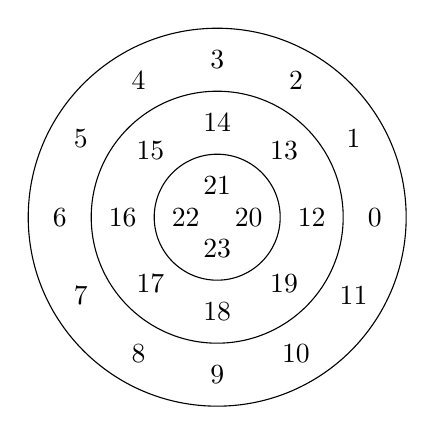
\begin{tikzpicture}
      \draw (0,0) circle (2.4cm);
      \draw (0,0) circle (1.6cm);
      \draw (0,0) circle (0.8cm);
      \foreach \i in {0,1,...,11}
      {
        \draw (\i*360/12: 2cm) node {\i};
      }
      \foreach \i in {12,13,...,19}
      {
        \draw (\i*360/8 - 180: 1.2cm) node {\i};
      }
      \foreach \i in {20,21,...,23}
      {
        \draw (\i*360/4: 0.4cm) node {\i};
      }
    \end{tikzpicture}
    \end{center}

    You may want to offset the sectors in different tracks so the head has
    time to settle

    \hspace{2em} Track skew allows the disk to be efficient with minimal head
    movement
  \end{frame}

  \begin{frame}{You May Want More Flexibility Than the Default Mapping}
    Pros

    \hspace{2em} Simple to program

    \hspace{2em} Default mapping reduces seek time for sequential access

    \vspace{2em}

    Cons

    \hspace{2em} Filesystem can't inspect or try to optimize the mapping

    \hspace{2em} Trying to reverse the mapping is difficult

    \hspace{4em} Number of sectors per track changes

    \hspace{4em} Disk silently remaps bad sectors
  \end{frame}

  \begin{frame}{A Cache Can Significantly Speed Up Disk Transfers}

    Disks have some internal memory (WD Red - 64 MB) for caching

    \vspace{2em}

    Implement a read-ahead ``track buffer''

    \hspace{2em} Read the entire contents of the track into memory during the rotational delay

    \vspace{2em}

    Write caching with volatile memory

    \hspace{2em} Write back: claim data is written to disk

    \hspace{4em} Fast, but there's data loss if there's a power failure

    \hspace{4em} Write through: acknowledge after data is physically written
  \end{frame}


  \begin{frame}{We Can Schedule Disk Accesses}

    We want to minimize the time the disk moves without reading or writing data

    \vspace{2em}

    FCFS: schedule requests in the order received

    \hspace{2em} Fair, but it has a high seek and rotation cost

    \vspace{2em}

    SSTF: shortest seek time first

    \hspace{2em} Handle the nearest cylinder/sector next

    \hspace{4em} Pro: reduces arm movement (seek time)

    \hspace{4em} Con: unfair, can starve some requests
  \end{frame}

  \begin{frame}{Elevator (aka SCAN or C-SCAN) Sweeps Across the Disk}
    \begin{center}
    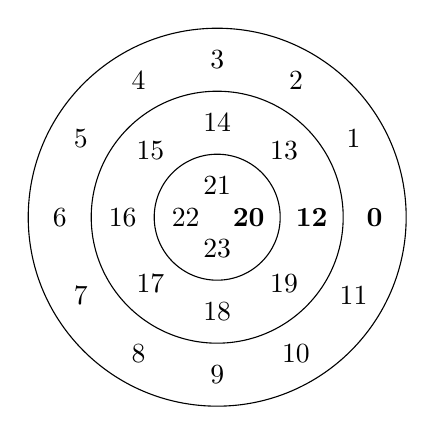
\begin{tikzpicture}
      \draw (0,0) circle (2.4cm);
      \draw (0,0) circle (1.6cm);
      \draw (0,0) circle (0.8cm);
      \draw (0: 2cm) node {\bf 0};
      \draw (0: 1.2cm) node {\bf 12};
      \draw (0: 0.4cm) node {\bf 20};
      \foreach \i in {1,...,11}
      {
        \draw (\i*360/12: 2cm) node {\i};
      }
      \foreach \i in {13,...,19}
      {
        \draw (\i*360/8 - 180: 1.2cm) node {\i};
      }
      \foreach \i in {21,...,23}
      {
        \draw (\i*360/4: 0.4cm) node {\i};
      }
    \end{tikzpicture}
    \end{center}

    If a request comes in for a track already serviced this sweep, queue it for
    the next
  \end{frame}

  \begin{frame}{Elevator (or SSTF) Ignores Rotation}
    \begin{center}
    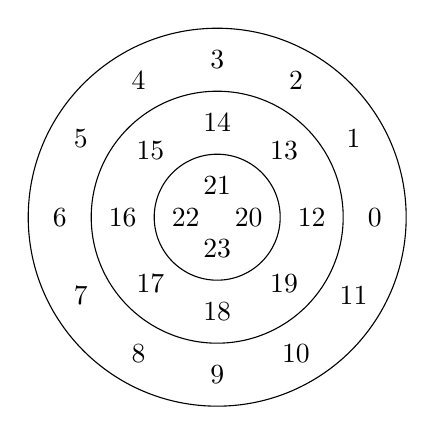
\begin{tikzpicture}
      \draw (0,0) circle (2.4cm);
      \draw (0,0) circle (1.6cm);
      \draw (0,0) circle (0.8cm);
      \foreach \i in {0,1,...,11}
      {
        \draw (\i*360/12: 2cm) node {\i};
      }
      \foreach \i in {12,13,...,19}
      {
        \draw (\i*360/8 - 180: 1.2cm) node {\i};
      }
      \foreach \i in {20,21,...,23}
      {
        \draw (\i*360/4: 0.4cm) node {\i};
      }
    \end{tikzpicture}
    \end{center}

    Shortest positioning time first (SPTF) is often the best strategy

    \hspace{2em} The OS and disk need to work together to implement this
  \end{frame}

  \begin{frame}{Solid State Drives (SSD) Are More Modern}

    Use transistors (like RAM) to store data rather than magnetic disks

    \vspace{2em}

    Pros

    \hspace{2em} No moving parts or physical limitations

    \hspace{2em} Higher throughput, and good random access

    \hspace{2em} More energy efficient

    \hspace{2em} Better space density

    \vspace{2em}

    Cons

    \hspace{2em} More expensive

    \hspace{2em} Lower endurance (number of writes)

    \hspace{2em} More complicated to write drivers for
  \end{frame}

  \begin{frame}{A SSD Contains Pages}
    \begin{center}
      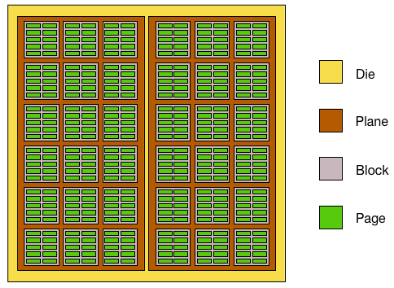
\includegraphics[height=0.8\textheight]{ssd.png}    
    \end{center}
  \end{frame}

  \begin{frame}{SSDs Using NAND Flash Are Much Faster Than HHDs}

    Pages are typically 4 KiB


    \vspace{2em}

    Reading a page: 10 μs

    Writing a page: 100 μs

    Erasing a block: 1 ms
  \end{frame}

  \begin{frame}{NAND Flash Programming Uses Pages and Blocks}

    You can only read complete pages and write to freshly erased pages

    \vspace{2em}

    Erasing is done per block (a block has 128 or 256 pages)

    \hspace{2em} An entire block needs to be erased before writing

    \vspace{2em}

    Writing is slow (may need to create a new block)
  \end{frame}

  \begin{frame}{The OS Can Help Speed Up SSDs}

    SSDs need to garbage collect blocks

    \hspace{2em} Move any pages that are still alive to a new block (may be overhead)

    \vspace{2em}

    The disk controller doesn't know what blocks are still alive

    \hspace{2em} SSD may think the disk is full, when a file could be deleted (not erased)

    \vspace{2em}

    The OS can use the \textit{TRIM} command to inform the SSD a block is unused

    \hspace{2em} The SSD can freely erase the block without moving overhead
  \end{frame}

  \begin{frame}{So Far We've Been Talking About Single Devices}

    Sometimes called Single Large Expensive Disk (SLED)

    \hspace{2em} Just one large disk for data

    \hspace{4em} Single point of failure

    \vspace{2em}

    There's also Redundant Array of Independent Disks (RAID)

    \hspace{2em} Data distributed on multiple disks

    \hspace{4em} Use redundancy to prevent data loss

    \hspace{4em} Use redundancy to increase throughput
  \end{frame}

  \begin{frame}{RAID 0 is Called a Striped Volume}

    Data stripes (128KB and 256KB) are distributed over disks

    \begin{center}
      \includesvg[height=5cm]{raid-0.svg}
    \end{center}
    
    \begin{flushright}
      by Cburnett licensed under CC BY-SA 3.0
    \end{flushright}
  \end{frame}

  \begin{frame}{RAID 0 is For Performance Only}

    The data is stripped across all disks in the array (you can have more than 2)

    \vspace{2em}

    Pro

    \hspace{2em} Faster parallel access, roughly $\mathsf{N}$ times speed

    \vspace{2em}

    Con

    \hspace{2em} Any disk failure results in a data loss (more points of failure)
  \end{frame}

  \begin{frame}{RAID 1 Mirrors All Data Across All Disks}

    \begin{center}
      \includesvg[height=5cm]{raid-1.svg}
    \end{center}

    \begin{flushright}
      by Cburnett licensed under CC BY-SA 3.0
    \end{flushright}
  \end{frame}

  \begin{frame}{RAID 1 is Simple, But Wasteful}

    Every disk in the array has a mirrored copy of all the data

    \vspace{2em}

    Pro

    \hspace{2em} Good reliability, as long as one disk remains, no data loss

    \hspace{2em} Good read performance

    \vspace{2em}

    Con

    \hspace{2em} High cost for redundancy (we can do better)

    \hspace{2em} Write performance is the same as a single disk
  \end{frame}

  \begin{frame}{RAID 4 Introduces Parity}

    Data stripes distributed over disks with a dedicated parity disk (p = parity)

    \hspace{2em} Parity stores xor $\oplus$ of copies 1-3, any one copy can be
                 reconstructed

    \begin{center}
      \includesvg[height=5cm]{raid-4.svg}
    \end{center}

    \begin{flushright}
      by Cburnett licensed under CC BY-SA 3.0
    \end{flushright}
  \end{frame}

  \begin{frame}{RAID 4 Can Use the Parity Drive to Recover}

    With parity, we can use $\mathsf{1 - \frac{1}{N}}$ of the available space

    \hspace{2em} Requires at least 3 drives

    \vspace{2em}

    Pro

    \hspace{2em} We get $\mathsf{(N - 1)}$ times performance
                 (removing parity disk)

    \hspace{2em} We can replace a failed disk and rebuild

    \vspace{2em}

    Con

    \hspace{2em} Write performance can suffer, every write must write to parity
                 disk
  \end{frame}

  \begin{frame}{RAID 5 Distributes Parity Across All Disks}

    Data stripes distributed over disks and each disk takes turns with parity
    blocks
    \begin{center}
      \includesvg[height=5cm]{raid-5.svg}
    \end{center}

    \begin{flushright}
      by Cburnett licensed under CC BY-SA 3.0
    \end{flushright}
  \end{frame}

  \begin{frame}{RAID 5 is an Improved Raid 4}

    It has all the same pros as RAID 4

    \vspace{2em}

    Write performance is improved, no longer a bottleneck on a single parity
    drive
  \end{frame}

  \begin{frame}{RAID 6 Adds Another Parity Block Per Stripe}
    \begin{center}
      \includesvg[height=5cm]{raid-6.svg}
    \end{center}

    \begin{flushright}
      by Cburnett licensed under CC BY-SA 3.0
    \end{flushright}
  \end{frame}

  \begin{frame}{RAID 6 Can Recover from 2 Simultaneous Drive Failures}

    Due to the extra parity, we can use $\mathsf{1 - \frac{2}{N}}$ of the available space

    \hspace{2em} Requires at least 4 drives

    \vspace{2em}

    Write performance is slightly less than RAID 5, due to another parity calculation
  \end{frame}

  \begin{frame}{Disks Enable Persistence}

    We explored two kinds of disks: SSDs and HDDs
    \begin{itemize}
      \item Magnetic disks have poor random access (need to be scheduled)
      \item Shortest Positioning Time First (SPTF) is the best scheduling for throughput
      \item SSDs are more like RAM except accessed in pages and blocks
      \item SSDs also need to work with the OS for best performance (TRIM)
      \item Use RAID to tolerate failures and improve performance using multiple disks
    \end{itemize}
  \end{frame}

\end{document}
